\section*{History}

\hbox{\begin{minipage}{0.80\textwidth}
\emph{\struct{{\Large If I have seen further than others,\\
it is by standing upon the shoulders of giants}}}\\
\mbox{}\hfill \emph{\struct{Isaac Newton}}
\end{minipage}\hspace{1em}
\begin{minipage}{0.15\textwidth}
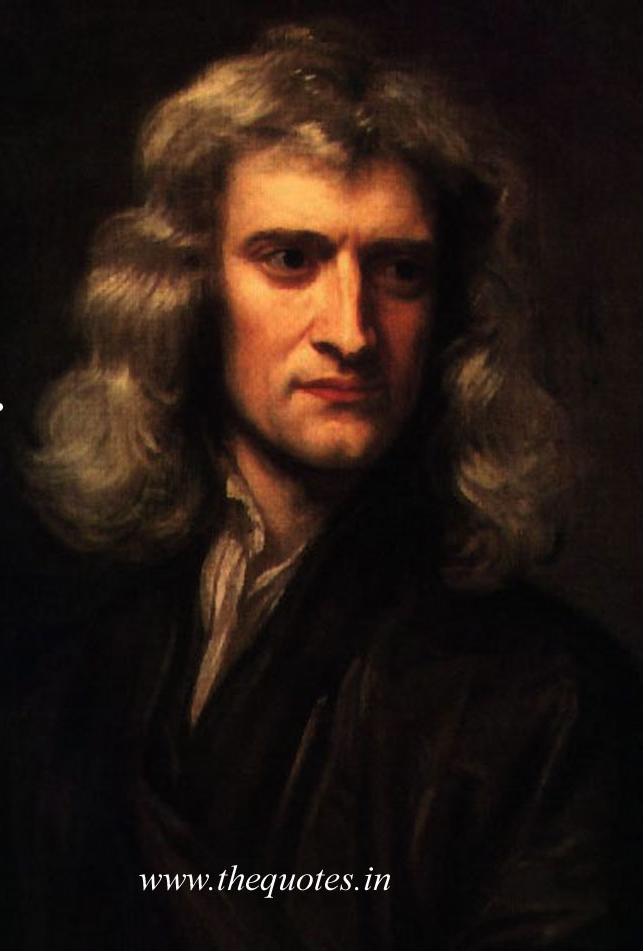
\includegraphics[scale=0.3]{I_Newton.jpg}
\end{minipage}}


Speaking about the history of UNIX and Linux we can recall the well-known
saying~--- \emph{we make our inventions stand on the shoulders of giants}.
But we must understand that many of these giants have failed.
But such fails can be a good lesson for new developers.

\medskip
\hbox{\begin{minipage}[b]{0.2\linewidth}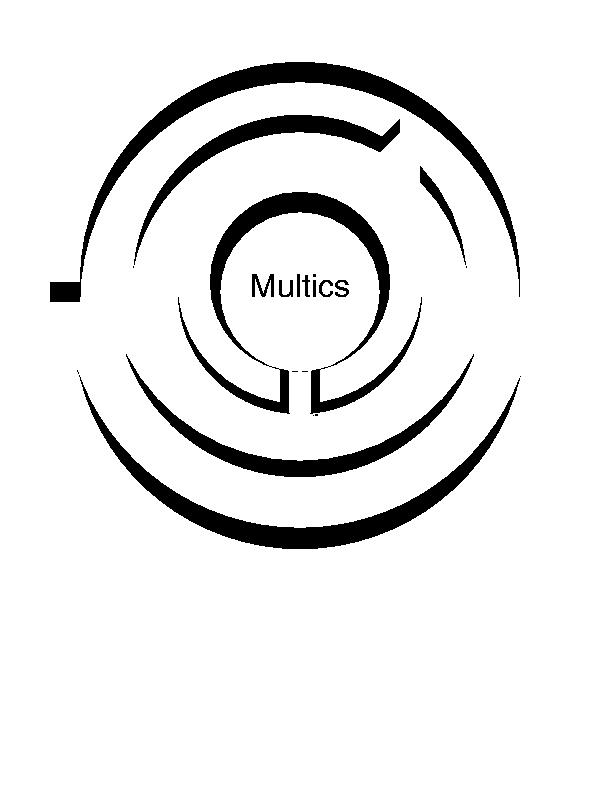
\includegraphics[scale=0.125]{Multics.png}
\end{minipage}
\begin{minipage}[b]{0.8\linewidth}
One such giant was the MULTICS project. The development of Multics began
in 1965 as a research project by MIT, General Electric and Bell Labs to create
a time-sharing, multiprocessing and multiuser interactive operating system.
After several years of development, the enthusiasm of the developers decreased
more and more as the system became more and more complex and the prospects
for completion of development became less and less.
\end{minipage}}

\medskip
\hbox{\begin{minipage}[b]{0.64\linewidth}
Bell Labs pulled out of the project in 1969; but some of the people
who worked on it got a lot of experience. Among them were \struct{Ken Thompson}
and \struct{Dennis Ritchie} of Bell Labs, the inventors of the \struct{UNIX OS}.
\end{minipage}\hspace{1em}
\begin{minipage}[b]{0.32\linewidth}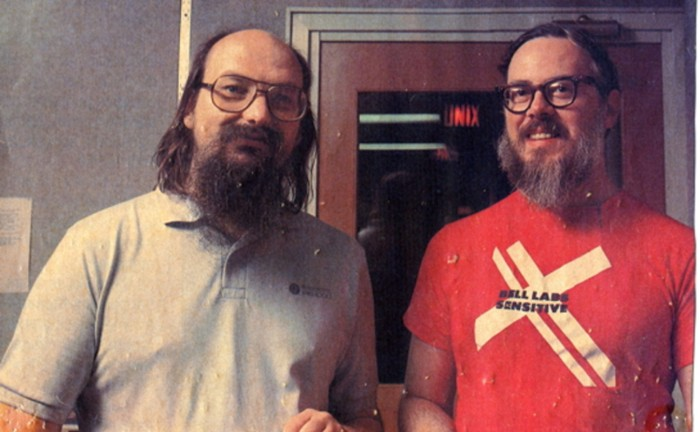
\includegraphics[scale=0.18]{thompson_ritchie.jpeg}
\end{minipage}
}

\medskip
\hbox{\begin{minipage}[b]{0.5\linewidth}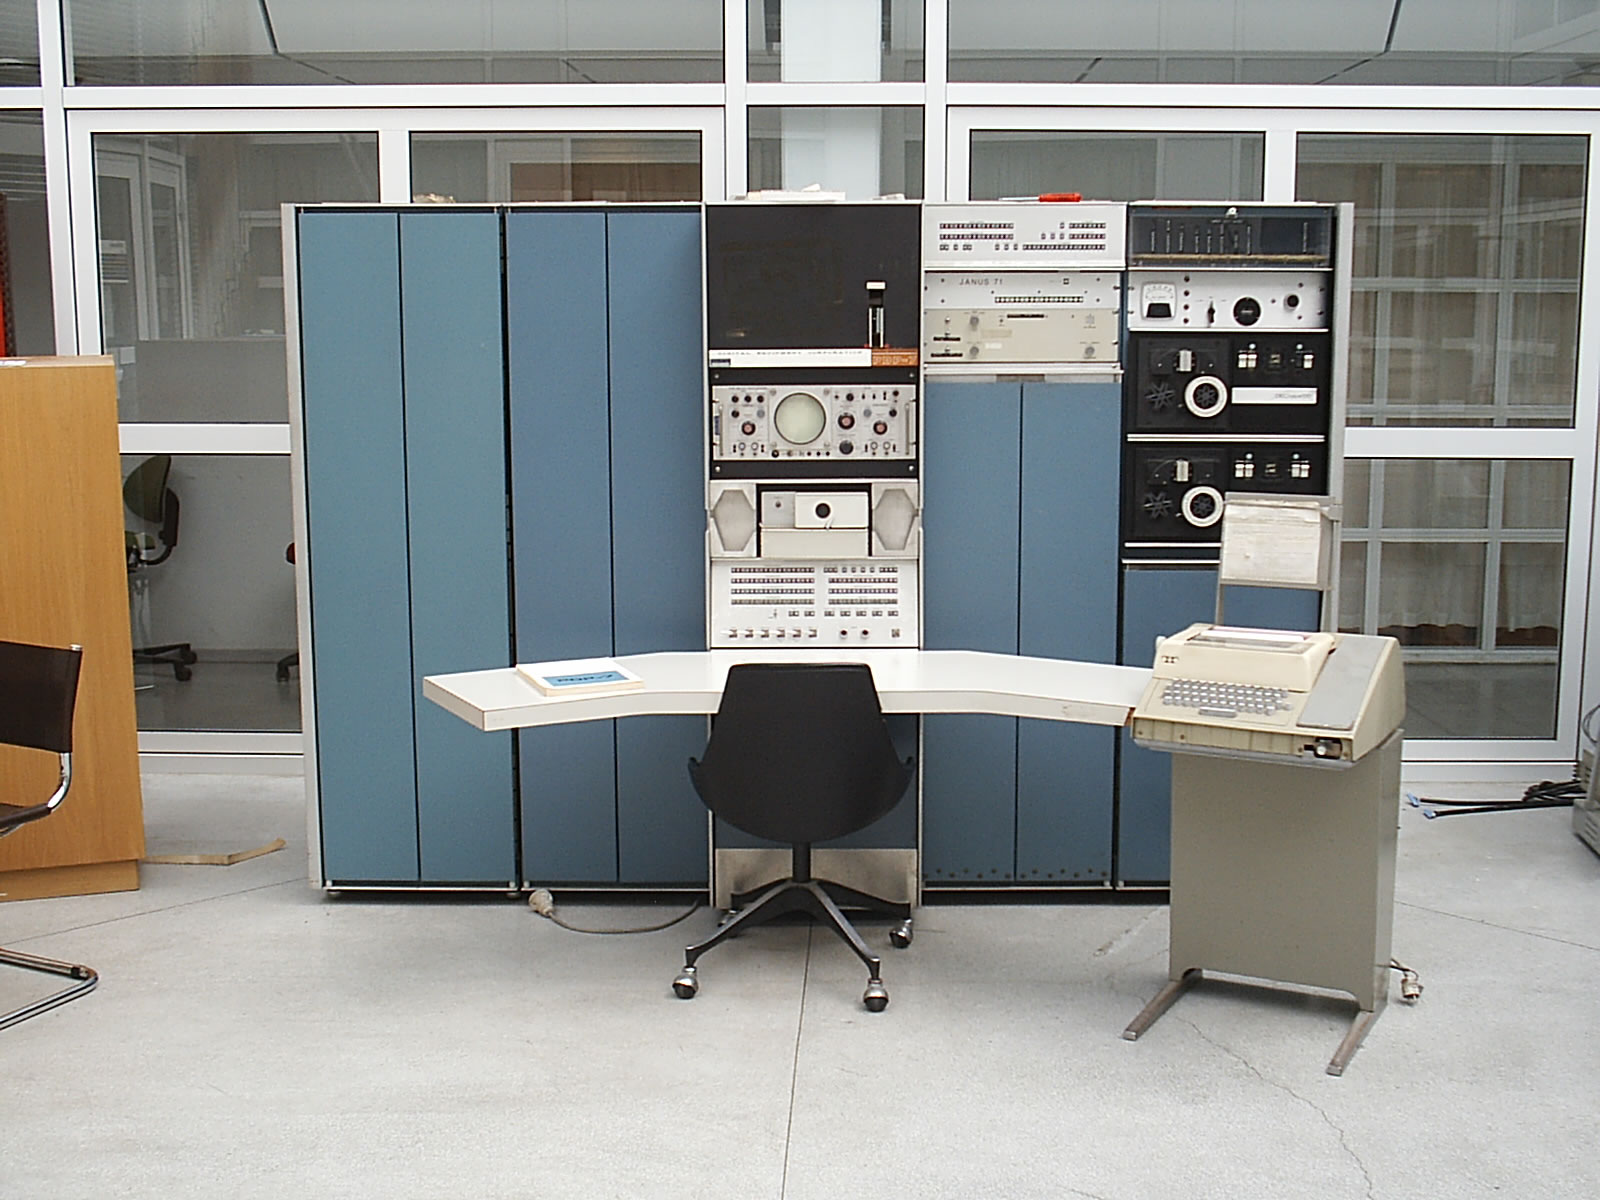
\includegraphics[scale=0.1]{Pdp7-oslo-2005.jpeg}
\end{minipage}\hspace{1em}
\begin{minipage}[b]{0.5\linewidth}
It's funny, but the history of Unix systems is closely related to computer games.
It started in 1969 when Ken Thompson discovered an old \mbox{PDP-7} computer
in a dark corner of the lab and wanted to use it to play Space Travel game.\\\\
\end{minipage}
}

%It's funny, but the history of Unix systems is closely related to computer games.
%It started in 1969 when Ken Thompson discovered an old \mbox{PDP-7} computer
%in a dark corner of the lab and wanted to use it to play Space Travel game.
\medskip
There was little to do~--- an operating system had to be written to run it.
And he did~--- at midnight on \struct{January 1, 1970}, the Unix epoch began.
From this time on, all clocks in UNIX-like systems count down the time,
including your mobile phone. Originally it was a single-tasking OS written
in assembly language that was loaded from paper tapes and called UNICS
as opposed to the complexity of MULTICS.

\href{http://www.levenez.com/unix/}{Unix History Timeline}

\hbox{\begin{minipage}[b]{0.65\linewidth}
And then the team of Ken Thompson and Dennis Ritchie received a new DEC PDP11
computer to develop a word processing system for the Bell Labs patent department.
For the first three months the machine sat in a corner, enumerating all
the closed Knight's tours on a $6\times8$ chess board~---
just because the hard drive wasn't shipped with a super new computer.
This time could be used to choose~a~programming language, because it was
a~computer with a completely new architecture and programs written on PDP7
assembler was not
\end{minipage}\hspace{1em}
\begin{minipage}[t]{0.35\linewidth}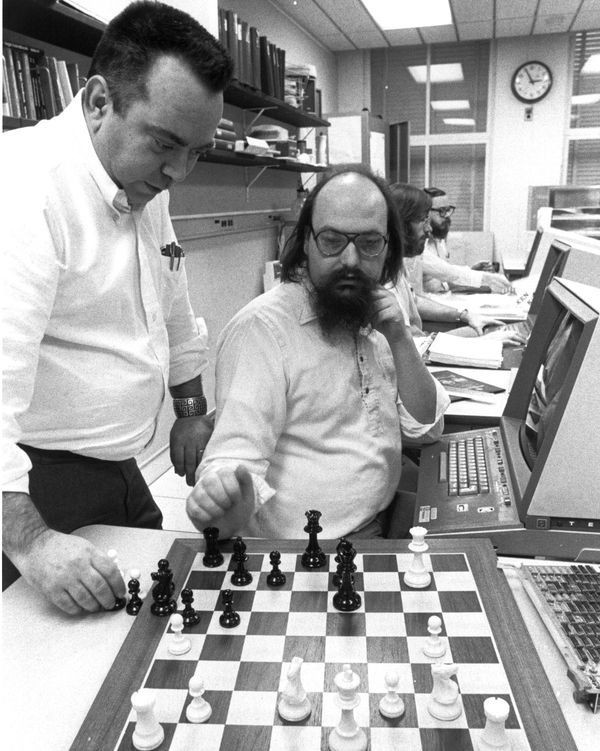
\includegraphics[scale=0.18]{chess.jpeg}
\end{minipage}
}

\noindent
useful for it. And most interesting was the concept of
another project used in some R\&D projects including MULTICS~--- \struct{BCPL}.
It was a high-level programming language focused on portability.
Most of this language was written in the language itself, and only a small
machine-dependent part was written in assembly. To support a new machine,
only 1/5 of the compiler code needed to be rewritten, which usually took
2-5 man-months.

\href{http://www.levenez.com/lang/}{Computer Languages History Timeline}

Thompson used the same concept when writing his simplified successor to BCPL,
language \struct{B}. This language was not very expressive and effective on
the \struct{PDP11}. In 1972, Ritchie started to improve B, which resulted in
creating a new language \struct{C}. In 1973, the UNIX kernel was refactored in C language
to follow the same concept of portability~--- most of the code was machine
independent.
%Finally, they got a very flexible and powerful system with
%a rich set of applications.
\begin{center}
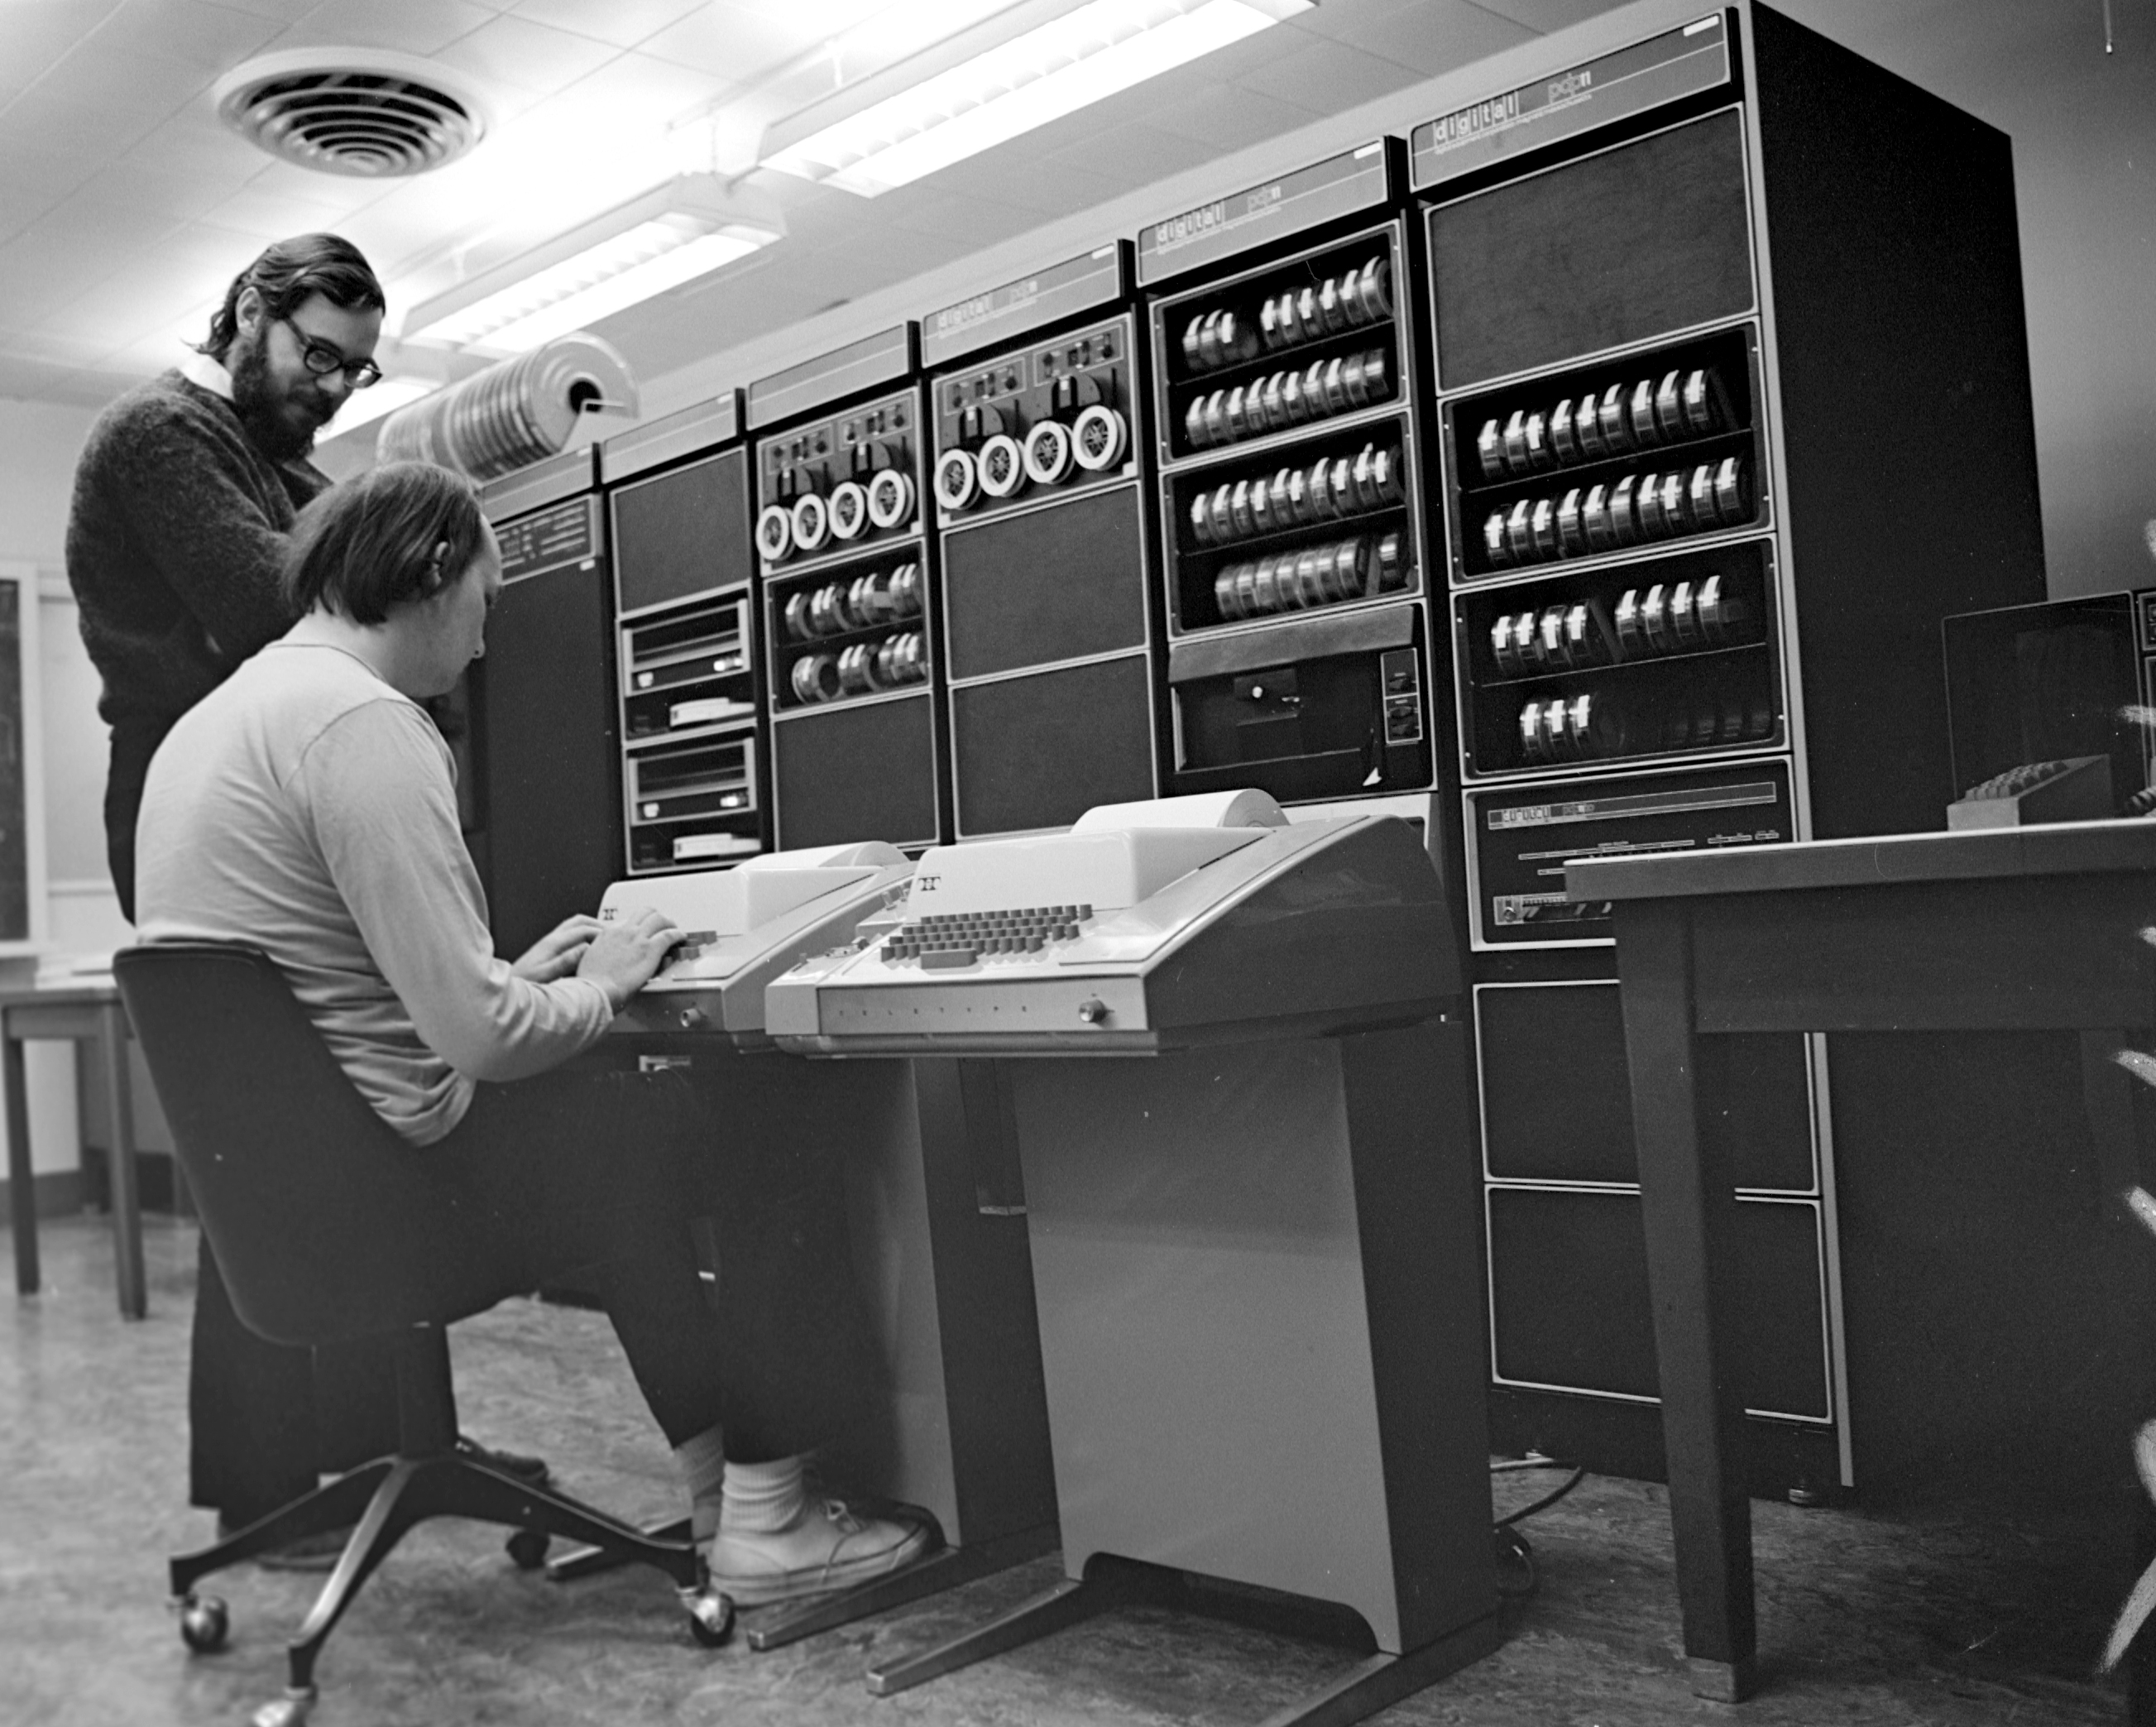
\includegraphics[scale=0.9]{Ken_Thompson__and_Dennis_Ritchie_at_PDP-11.jpg}
\end{center}

The system was distributed in source code among universities for a nominal fee,
which served as an explosive growth in its popularity in the 80s.
Almost all the developers of new computer systems since this period have used
UNIX as the base platform for their new developments. One of the most famous of
these is the Berkeley Software Distribution (\struct{BSD}) developed at
the University of California, Berkeley based on \struct{Unix version 6}
with its \struct{own copyleft license}. And most of the hardware vendors of
the 1980s used BSD as the base OS for their new computers.

UNIX was not a significant part of AT\&T Bell Laboratories' business,
and it was not a problem for them. But in the 1980s Bell Labs split
into several companies as a result of an antitrust lawsuit against AT\&T.
The new UNIX System Laboratories company was created and the new
\struct{UNIX System V} specification was developed. UNIX was the main business
of this company, and they were very aggressive in pushing the new standard in
the market. And that has been the cause of \struct{UNIX wars} against
\struct{non-commercial developers} including BSD.

The commercialization of the UNIX system market and the move to a closed
development and distribution model has led to an alternative movement~---
\struct{GNU}. What is GNU? You know, it's such an African animal. But also it
is a self-referential abbreviation ``\struct{G}NU is \struct{N}ot \struct{U}nix''.
Richard Stallman founded the project in 1978 at MIT. The GNU project is a mass
collaborative initiative for the development of free software. The first
goal of this project was to develop a set of programs similar to
the standard set of utilities in UNIX.

In 1991, a Finnish student \struct{Linus Torvalds} created his own operating
system kernel, which is compatible with the UNIX OS, called \struct{Linux}.
As he said later, ``Just for fun''. The Linux kernel, combined with the set of
utilities from the GNU project, served as the basis for creating a complete
operating system, comparable in capabilities to commercial UNIX systems,
and usually even superior to them.

\medskip
\href{https://www.bell-labs.com/usr/dmr/www/hist.html}%
{\url{https://www.bell-labs.com/usr/dmr/www/hist.html}}

\noindent
\href{https://www.bell-labs.com/usr/dmr/www/chist.html}%
{\url{https://www.bell-labs.com/usr/dmr/www/chist.html}}
